%!Mode:: "TeX:UTF-8"
\documentclass[a4paper,11pt,UTF8]{ctexart}

\usepackage{indentfirst} %缩进
\usepackage{xeCJK}    %使用系统字体
\usepackage{bm}       %粗体
\usepackage{fancyhdr} %自定义页眉页脚
\pagestyle{empty}                   %不设置页眉页脚
\usepackage{amsmath, amsthm, amssymb, amsfonts} %数学公式
\usepackage[a4paper,left=3cm,right=3cm,top=3.5cm,bottom=3.5cm]{geometry}
\usepackage{booktabs} %插入表格
\usepackage[section]{placeins} %避免浮动
\usepackage{listings} %插入代码
\usepackage{ctex}     %中文宏包
\usepackage[svgnames, table]{xcolor} %彩色表格
\usepackage{algorithm}          %伪代码
\usepackage{algorithmicx}
\usepackage{algpseudocode}
\usepackage{algorithm,algpseudocode,float}
\usepackage{lipsum}
\usepackage{enumitem}           %调整列举环境
\usepackage{url}
\usepackage{fontspec,xunicode}
\defaultfontfeatures{Mapping=tex-text} %如果没有它,会有一些 tex 特殊字符无法正常使用,比如连字符。

\usepackage{graphicx}
\graphicspath{{imgs/}}

%%%%%%%%%%%%%%%%%%%%%%%%%%%%%%%%%%%%%%%%%%%%%%%%%%%%%%%%%%%%%%%%
% 缩进及行间距
%%%%%%%%%%%%%%%%%%%%%%%%%%%%%%%%%%%%%%%%%%%%%%%%%%%%%%%%%%%%%%%%
\setlength{\parindent}{22bp} %重新定义缩进长度
\linespread{1}

%%%%%%%%%%%%%%%%%%%%%%%%%%%%%%%%%%%%%%%%%%%%%%%%%%%%%%%%%%%%%%%%
% 图的标题行间距设置
%%%%%%%%%%%%%%%%%%%%%%%%%%%%%%%%%%%%%%%%%%%%%%%%%%%%%%%%%%%%%%%%
\newcommand{\bottomcaption}{%
\setlength{\abovecaptionskip}{6bp}%
\setlength{\belowcaptionskip}{6bp}%
\caption}


%%%%%%%%%%%%%%%%%%%%%%%%%%%%%%%%%%%%%%%%%%%%%%%%%%%%%%%%%%%%%%%%
% 字体定义
%%%%%%%%%%%%%%%%%%%%%%%%%%%%%%%%%%%%%%%%%%%%%%%%%%%%%%%%%%%%%%%%
\setmainfont{Times New Roman}  %默认英文字体.serif是有衬线字体sans serif无衬线字体
\setmonofont{Consolas}
\setCJKmainfont[ItalicFont={楷体}, BoldFont={黑体}]{宋体}%衬线字体 缺省中文字体为
\setCJKsansfont{黑体}
\punctstyle{hangmobanjiao}
%-----------------------xeCJK下设置中文字体------------------------------%
\setCJKfamilyfont{song}{SimSun}                             %宋体 song
\newcommand{\song}{\CJKfamily{song}}
\setCJKfamilyfont{fs}{FangSong}                      %仿宋  fs
\newcommand{\fs}{\CJKfamily{fs}} 
\let\kaishu\relax                                    %重定义楷体,打开假粗体
\newCJKfontfamily\kaishu{KaiTi}[AutoFakeBold] 
%\setCJKfamilyfont{ktgb}{KaiTi_GB2312}                      %楷体 GB2312
%\newcommand{\ktgb}{\CJKfamily{ktgb}}
\setCJKfamilyfont{yh}{Microsoft YaHei}                    %微软雅黑 yh
\newcommand{\yh}{\CJKfamily{yh}}
\setCJKfamilyfont{hei}{SimHei}                              %黑体  hei
\newcommand{\hei}{\CJKfamily{hei}}
\setCJKfamilyfont{hwxk}{STXingkai}                                %华文行楷  hwxk
\newcommand{\hwxk}{\CJKfamily{hwxk}}
%------------------------------设置字体大小------------------------%
\newcommand{\chuhao}{\fontsize{42bp}{63bp}\selectfont}     %初号, 1.5倍行距
\newcommand{\xiaochuhao}{\fontsize{36bp}{36bp}\selectfont} %小初号,单倍行距
\newcommand{\yihao}{\fontsize{26bp}{39bp}\selectfont}        % 一号, 1.5 倍行距
\newcommand{\erhao}{\fontsize{22bp}{33bp}\selectfont}        % 二号, 1.5倍行距
\newcommand{\xiaoerhao}{\fontsize{18bp}{18bp}\selectfont}       % 小二, 单倍行距
\newcommand{\sanhao}{\fontsize{16bp}{24bp}\selectfont}       % 三号, 1.5倍行距
\newcommand{\xiaosanhao}{\fontsize{15bp}{22bp}\selectfont}      % 小三, 1.5倍行距
\newcommand{\sihao}{\fontsize{14bp}{21bp}\selectfont}        % 四号, 1.5 倍行距
\newcommand{\banxiaosi}{\fontsize{13bp}{20bp}\selectfont}  % 半小四, 20pt行距
\newcommand{\xiaosihao}{\fontsize{12bp}{20bp}\selectfont}       % 小四, 20pt行距
\newcommand{\dawuhao}{\fontsize{11bp}{11bp}\selectfont}      % 大五号, 单倍行距
\newcommand{\wuhao}{\fontsize{10.5bp}{10.5bp}\selectfont}   % 五号, 单倍行距
\newcommand{\xiaowuhao}{\fontsize{9bp}{9bp}\selectfont}   %小五号,单倍行距
%------------------------------重定义normalize------------------------%
\renewcommand{\normalsize}{\fontsize{12bp}{20bp}\selectfont}


%%%%%%%%%%%%%%%%%%%%%%%%%%%%%%%%%%%%%%%%%%%%%%%%%%%%%%%%%%%%%%%%
% 图题字体大小相同
%%%%%%%%%%%%%%%%%%%%%%%%%%%%%%%%%%%%%%%%%%%%%%%%%%%%%%%%%%%%%%%%
\usepackage{caption}
\captionsetup{font={footnotesize}}   % footnotesize = 9bp
\captionsetup[lstlisting]{font={footnotesize}}

%%%%%%%%%%%%%%%%%%%%%%%%%%%%%%%%%%%%%%%%%%%%%%%%%%%%%%%%%%%%%%%%
% 重定义枚举编号为 1),2)...
%%%%%%%%%%%%%%%%%%%%%%%%%%%%%%%%%%%%%%%%%%%%%%%%%%%%%%%%%%%%%%%%
\renewcommand{\labelenumi}{\theenumi)}


%%%%%%%%%%%%%%%%%%%%%%%%%%%%%%%%%%%%%%%%%%%%%%%%%%%%%%%%%%%%%%%%
% 重定义section标题
%%%%%%%%%%%%%%%%%%%%%%%%%%%%%%%%%%%%%%%%%%%%%%%%%%%%%%%%%%%%%%%%
\CTEXsetup[format={\CJKfamily{zhhei}\zihao{4}},number={\chinese{section}},name={,、~},aftername={},indent={0bp},beforeskip={6bp},afterskip={6bp},format+={\flushleft}]{section}
\CTEXsetup[format={\Large\bfseries\CJKfamily{zhkai}\zihao{5}},name={(,)},number={\chinese{subsection}},aftername={},indent={22bp},beforeskip={6bp},afterskip={6bp}]{subsection}
\CTEXsetup[number={\chinese{section}},name={附录, ~~ }]{appendix}



%%%%%%%%%%%%%%%%%%%%%%%%%%%%%%%%%%%%%%%%%%%%%%%%%%%%%%%%%%%%%%%%
% 标题名称中文化
%%%%%%%%%%%%%%%%%%%%%%%%%%%%%%%%%%%%%%%%%%%%%%%%%%%%%%%%%%%%%%%%
\renewcommand\figurename{\hei 图}
\renewcommand\tablename{\hei 表}
\renewcommand\lstlistingname{\hei 代码}
\renewcommand{\algorithmicrequire}{\textbf{输入:}}
\renewcommand{\algorithmicensure}{\textbf{输出:}}
\newtheorem{define}{定义}


%%%%%%%%%%%%%%%%%%%%%%%%%%%%%%%%%%%%%%%%%%%%%%%%%%%%%%%%%%%%%%%%
% 列表设置
%%%%%%%%%%%%%%%%%%%%%%%%%%%%%%%%%%%%%%%%%%%%%%%%%%%%%%%%%%%%%%%%
\setlist[enumerate,1]{itemindent=22bp,listparindent=\parindent,itemsep=0mm,partopsep=.7mm,parsep=0ex,labelsep=1.5mm,topsep=0.7mm}
\setlist[enumerate,2]{label=\alph*),leftmargin=1.5em}  %二级item设置
%\setitemize{itemindent=38bp,leftmargin=0bp,itemsep=-0.4ex,listparindent=26bp,partopsep=0bp,parsep=0.5ex,topsep=-0.25ex}
%\setdescription{itemindent=38bp,leftmargin=0bp,itemsep=-0.4ex,listparindent=26bp,partopsep=0bp,parsep=0.5ex,topsep=-0.25ex}

%%%%%%%%%%%%%%%%%%%%%%%%%%%%%%%%%%%%%%%%%%%%%%%%%%%%%%%%%%%%%%%%
% 代码设置
%%%%%%%%%%%%%%%%%%%%%%%%%%%%%%%%%%%%%%%%%%%%%%%%%%%%%%%%%%%%%%%%
\lstset{
 columns=fixed,
 numbers=left,                                        % 在左侧显示行号
 numberstyle=\tiny\color{gray},                       % 设定行号格式
 frame=single,                                        % 单线背景边框
 breaklines=true,                                     % 设定LaTeX对过长的代码行进行自动换行
 keywordstyle=\color[RGB]{40,40,255},                 % 设定关键字颜色
 numberstyle=\footnotesize\color{darkgray},
 commentstyle=\it\color[RGB]{0,96,96},                % 设置代码注释的格式
 stringstyle=\rmfamily\slshape\color[RGB]{128,0,0},   % 设置字符串格式
 showstringspaces=false,                              % 不显示字符串中的空格
 language=java,                                        % 设置语言
 basicstyle=\linespread{1.0}\xiaowuhao\ttfamily,                      % 字体字号
 %lineskip=10bp,
 %baselinestretch=1,
}

%%%%%%%%%%%%%%%%%%%%%%%%%%%%%%%%%%%%%%%%%%%%%%%%%%%%%%%%%%%%%%%%
% 伪代码分页
%%%%%%%%%%%%%%%%%%%%%%%%%%%%%%%%%%%%%%%%%%%%%%%%%%%%%%%%%%%%%%%%
\makeatletter
\renewcommand{\ALG@name}{算法}
\newenvironment{breakablealgorithm}
  {% \begin{breakablealgorithm}
   \begin{center}
     \refstepcounter{algorithm}% New algorithm
     \hrule height.8bp depth0bp \kern2bp% \@fs@pre for \@fs@ruled
     \renewcommand{\caption}[2][\relax]{% Make a new \caption
       {\raggedright\textbf{\ALG@name~\thealgorithm} ##2\par}%
       \ifx\relax##1\relax % #1 is \relax
         \addcontentsline{loa}{algorithm}{\protect\numberline{\thealgorithm}##2}%
       \else % #1 is not \relax
         \addcontentsline{loa}{algorithm}{\protect\numberline{\thealgorithm}##1}%
       \fi
       \kern2bp\hrule\kern2bp
     }
  }{% \end{breakablealgorithm}
     \kern2bp\hrule\relax% \@fs@post for \@fs@ruled
   \end{center}
  }
\makeatother



\begin{document}
\xiaosihao\song

\begin{titlepage}
    \center{\yihao{\hwxk{2021年电子科技大学盟升杯电子设计竞赛}}}
    \vspace{6cm}
    \center{\xiaochuhao{\kaishu{\bfseries 设~计~报~告}}}
    \center{\yihao{\kaishu{\bfseries D题 ~多功能闹钟}}}
    \vspace{4cm}

    \vfill \hfill
\end{titlepage}
\clearpage

\centerline{\\[10bp]\erhao{\fs{2021年电子科技大学盟升杯电子设计竞赛}}}

\centerline{\\[20bp]\yihao{\fs{设 ~~~~计 ~~~~报 ~~~~告}}}

\leftline{\\[10bp]\sihao{\hei{\hspace{1.5em} 题目:新生组D题 ~多功能小车 \hfill }}}

\setlength{\parskip}{0bp}  %定义段间距

\section{摘要}

本小组制作的多功能闹钟主要由STM32单片机最小系统、数码管模块、按键模块、光敏电阻模块、稳压电源模块、蜂鸣器模块、DHT11温湿度传感器模块和备用电池模块组成。本设计采用了双层洞洞板设计,STM32单片机最小系统板、稳压电源、备用电池位于下层板,数码管、按钮、光敏电阻、温湿度传感器和蜂鸣器等交互模块位于上层板,上下两层板通过排针连接,整体结构设计合理,空间利用率高。用户能通过上下左右四个按键直观地与本作品进行交互,能通过LED数码管显示的功能菜单完成时间设置、温湿度查看、闹钟设置等功能。本作品内置了几首蜂鸣器音乐用户选择作为闹钟铃声。除题目要求的功能外,本作品还实现了秒表和倒计时功能。本组的设计能较好地完成多功能闹钟的任务。

\section{系统方案}

\subsection{电路载体选择}

\begin{enumerate}
    \item 单层洞洞板
    \item 双层洞洞板
    \item PCB
\end{enumerate}

选择:(3)

分析:单层洞洞板设计、制作和调试难度均较低,但空间利用率不高,不够美观;双层洞洞板将不与用户交互的模块置于背面,同时提供额外空间进行走线,但设计、制作和调试较为复杂;PCB能提供最稳定和美观的效果,但是设计、加工、调试周期较长,成本较高。综合考虑各种因素后,我们选择使用双层洞洞板。

\subsection{供电选择}

\begin{enumerate}
    \item 自治LM7805 9V转5V稳压电源模块
    \item USB 5V电源输入
    \item 调试端口3V3电源输入
\end{enumerate}

选择:(1)(2)(3)

分析:题目要求采用(1)方式供电,但最小系统板自带后两种供电方式支持,配置较为方便。

\subsection{按钮输入方式选择}

\begin{enumerate}
    \item 开漏输出
    \item 推挽输出,上拉输入
\end{enumerate}

选择:(2)

分析:开漏输入需要手动连接上拉电阻,方案2通过软件切换GPIO引脚的输入方式,可免去上拉电阻,电路设计更加简洁,故采用方案2。

\subsection{小结}

经过小组同学的讨论,我们决定选择在双层洞洞板上制作作品,同时采用三种供电方式,使用上拉电阻模式连接按钮,通过切换GPIO模式控制DHT11的创新设计方案。

\section{理论分析与计算}

\subsection{系统结构的分析}

\subsubsection{系统理论}

通过对题目要求的分析,多功能闹钟是一个以STM32单片机最小系统为控制核心且外附各类组件以完成各项功能的系统。需要外接进行控制的模块有:数码管模块、按键模块、光敏电阻模块、蜂鸣器模块和DHT11温湿度传感器模块。

\subsubsection{数码管模块理论}

直接将单片机GPIO引脚连接数码管阳极和阴极,每次将共阴数码管的一个阴极置为低电平,其余为高电平,将数码需点亮的笔画的阳极置于高电平,其余阳极为低电平,来点亮一位数码,编程控制快速依次点亮四位数码达到同时显示四位数码的效果。为实现显示亮度调节,将阴极四个引脚连接到STM32的定时器PWM输出引脚,通过改变PWM占空比实现亮度调节。

\subsubsection{按键模块理论}

将四个按钮的一端与单片机的四个上拉输入引脚相连,另一端接地。单片机每隔一定时间检测一次按钮引脚电位,按钮未按下时处于高电位,按下时处于低电位。为实现按键防抖,只有连续几次探测到低电位时才出发按键处理程序。

\subsubsection{光敏电阻模块理论}

将光敏电阻与一定大小的电阻串联后接在VCC与GND之间,利用单片机ADC检测光敏电阻和定值电阻之间的电压,即可根据串联分压原理获取光敏电阻阻值,进而获得光线强度。

\subsubsection{蜂鸣器模块理论}

采用无源蜂鸣器,向蜂鸣器施加PWM方波电压即可控制蜂鸣器发声及发生频率。编程连续按照录入的乐谱改变频率即可实现音乐播放。由于蜂鸣器正常工作时电压和电流较大,而单片机引脚输出电流电压有限,需通过三极管放大电流。

\subsubsection{DHT11温湿度传感器模块理论}

DHT11温湿度传感器通过数字方式与STM32主机通信,查阅其技术手册可获得读取数据所用的具体通讯协议,编程实现该协议即可。

\subsection{相关计算}

\subsubsection{数码管LED限流电阻}

单片机引脚输出电压为3.3V,LED工作电流约2mA,正向电压约2.6V,计算得需串联约$260\Omega$的电阻,通过并联两个$350\Omega$电阻来近似实现。

\subsubsection{与光敏电阻串联的电阻}

用万用表测得光敏电阻在阴天太阳光下电阻约$2k\Omega$,完全遮挡约$18k\Omega$ ,串联一个$3.5k\Omega$的电阻可以明显测量两端电压变化。

\subsubsection{音乐播放}

使用状态机模型驱动音乐播放程序,规定每秒调用音乐播放程序50次,结合音乐节奏计算,可得约3次循环播放一个十六分音符较为适合。SysTick计时器频率为8MHz,除以每个音高的标准频率可计算PWM周期。

\section{电路设计}

\subsection{系统总体框图}

系统总体框图已由题目要求给出。

\begin{figure}[!htbp]
    \centering
    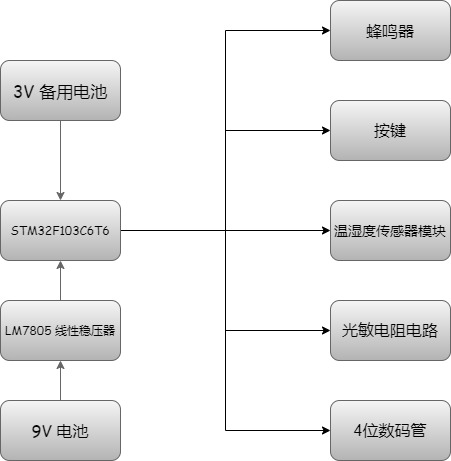
\includegraphics[width=10cm]{image1.png}
    \bottomcaption{\xiaowuhao{系统总体框图}}
\end{figure}

下面是各个模块的电路原理图。

\subsection{稳压电源模块}

\begin{figure}[!htbp]
    \centering
    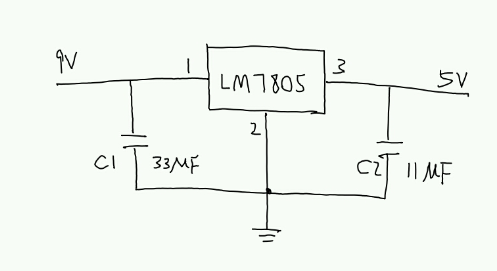
\includegraphics[width=6cm]{image2.png}
    \bottomcaption{\xiaowuhao{稳压电源模块原理图}}
\end{figure}

其中C1电容用三个$10μF$电容并联代替。

\subsection{备用电池模块}

\begin{figure}[!htbp]
    \centering
    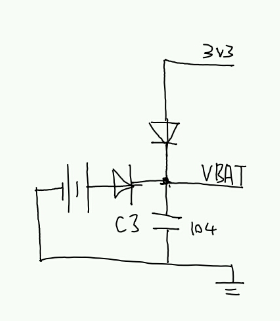
\includegraphics[width=6cm]{image3.png}
    \bottomcaption{\xiaowuhao{备用电池模块原理图}}
\end{figure}

通过二极端接入3.3V输入,允许主电源接通时不消耗备用电池。使用一个104滤波电容。

\subsection{蜂鸣器模块}

\begin{figure}[!htbp]
    \centering
    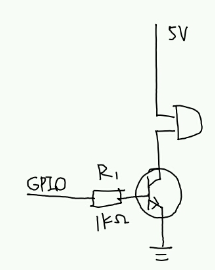
\includegraphics[width=6cm]{image4.png}
    \bottomcaption{\xiaowuhao{蜂鸣器模块原理图}}
\end{figure}

使用NPN型三极管S8050在接地端控制电流。

\subsection{按键模块}

\begin{figure}[!htbp]
    \centering
    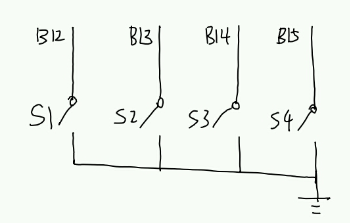
\includegraphics[width=6cm]{image5.png}
    \bottomcaption{\xiaowuhao{按键模块原理图}}
\end{figure}

按键一端接单片机上拉输入引脚,一端接地。

\subsection{DHT11温湿度传感器模块}

\begin{figure}[!htbp]
    \centering
    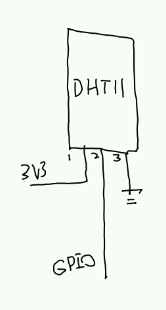
\includegraphics[width=4cm]{image6.png}
    \bottomcaption{\xiaowuhao{DHT11温湿度传感器模块原理图}}
\end{figure}

成品DHT11模块已包含电源滤波电容,直接将数据线连接单片机GPIO。

\subsection{光敏电阻模块}

\begin{figure}[!htbp]
    \centering
    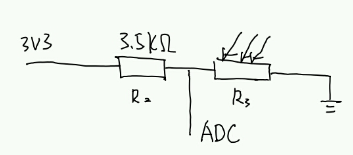
\includegraphics[width=6cm]{image7.png}
    \bottomcaption{\xiaowuhao{光敏电阻模块原理图}}
\end{figure}

光敏电阻阻值随光强减小,则ADC读取的电压值与光照强度负相关。

\subsection{LED数码管模块}

\begin{figure}[!htbp]
    \centering
    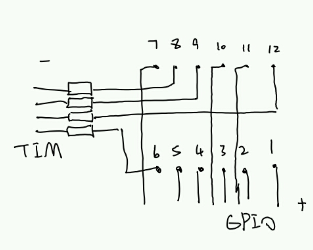
\includegraphics[width=6cm]{image8.png}
    \bottomcaption{\xiaowuhao{LED数码管模块原理图}}
\end{figure}

12个管脚均直接由单片机GPIO控制。由于阴极数量较少,将限流电阻设置在阴极,并将阴极连接到带PWM输出功能的引脚实现亮度调节。

\begin{figure}[!htbp]
    \centering
    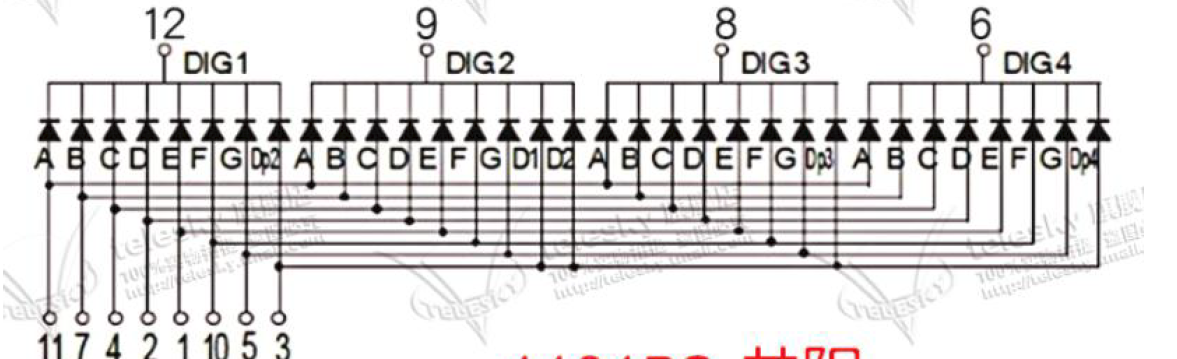
\includegraphics[width=\textwidth]{image9.png}
    \bottomcaption{\xiaowuhao{数码管内部原理图}}
\end{figure}

\subsection{各模块与STM32核心板连接}

\subsubsection{单层洞洞板方案}

我们论证了该方案的可行性,并做出了洞洞板布局设计,但并未实际使用。

\begin{figure}[!htbp]
    \centering
    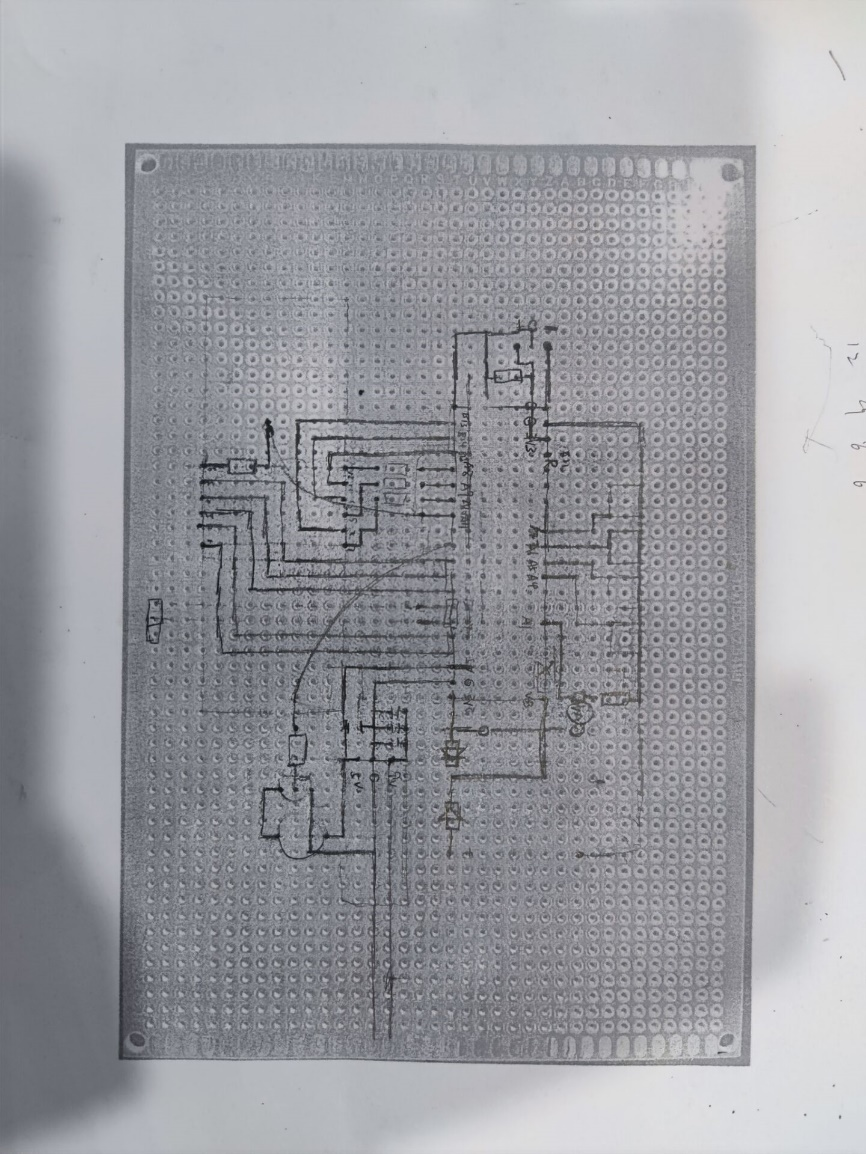
\includegraphics[width=8cm, angle=270]{image10.jpeg}
    \bottomcaption{\xiaowuhao{单层洞洞板设计图}}
\end{figure}

\subsubsection{双层洞洞板方案}

\begin{figure}[!htbp]
    \centering
    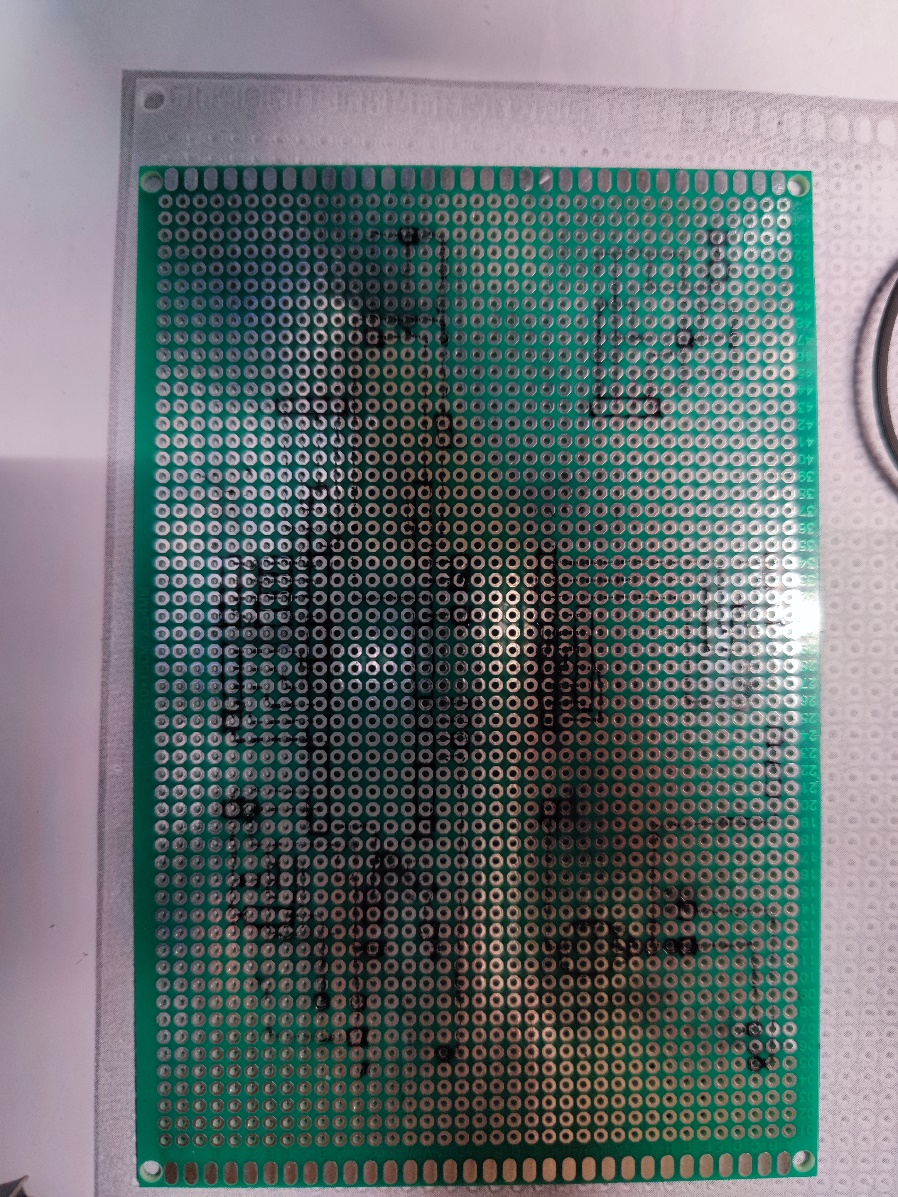
\includegraphics[width=8cm, angle=270]{image11.jpeg}
    \bottomcaption{\xiaowuhao{双层洞洞板设计图}}
\end{figure}

方便起见,我们直接在洞洞板上绘制了线路连接方案,整体采用紧凑型设计,仅使用一条飞线,其余电路均通过焊锡连接。完成元件焊接和线路焊接后,用美工刀沿中线裁开洞洞板,再利用排针完成上下两层板,下层板和单片机核心板之间的物理连接和电气连接,排针两端均焊死以提升结构强度。主电源开关通过向外弯折的排针固定在下层板侧边。

\begin{figure}[!htbp]
    \centering
    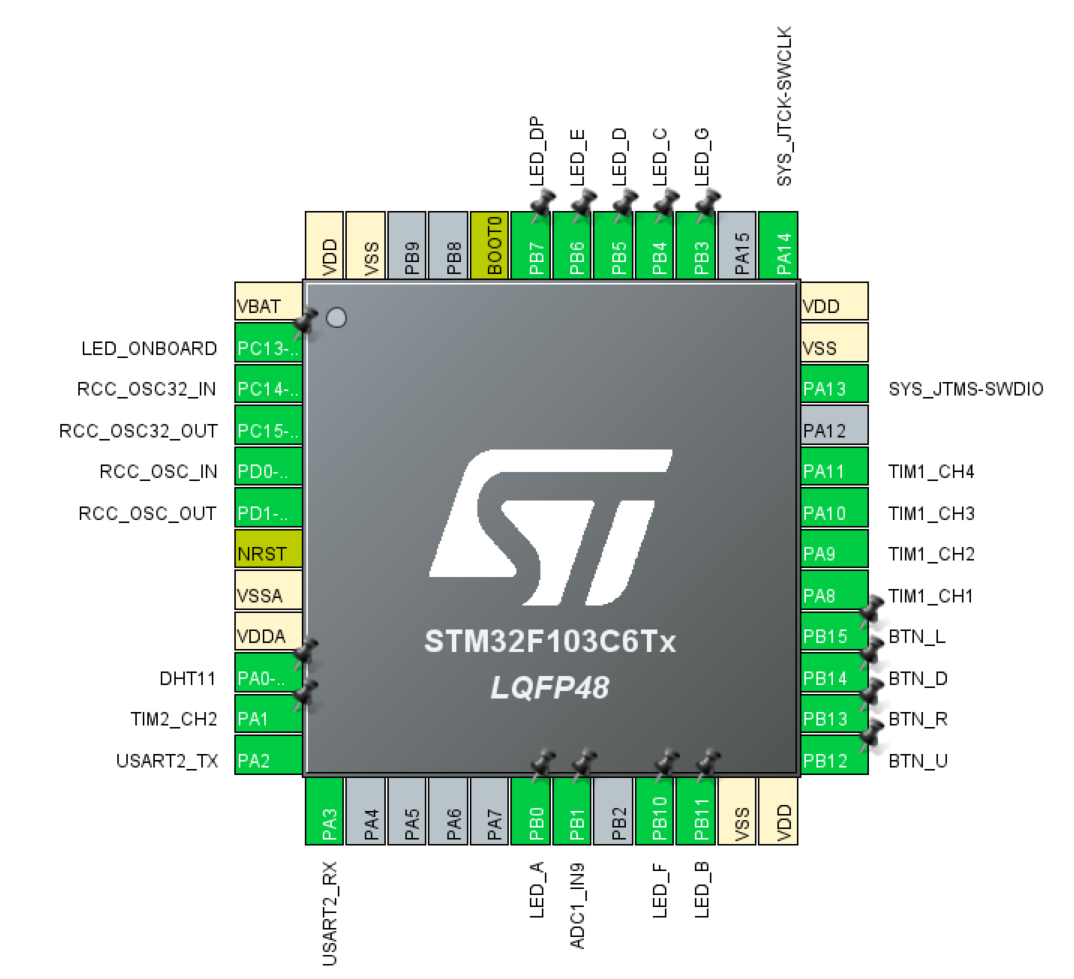
\includegraphics[width=10cm]{image12.png}
    \bottomcaption{\xiaowuhao{CubeMX管脚配置}}
\end{figure}

\section{测试方案与结果}

\subsection{方案论证测试}

在正式制作开始前,我们制作了一块测试板,通过杜邦线与单片机连接进行各模块测试。

\subsection{单元测试}

在连接单片机前,将各模块与稳压电源、函数发生器和多用电表等仪器相连,模拟输入,检测其是否工作正常。

LED数码管:将稳压电源调为3.3V,分别于每个阳极和阴极相连,观察到每个数码管笔画均能正常发光。

按钮:将多用电表设置为蜂鸣模式,两表笔接于开关两端,按下按钮时多用电表能发出蜂鸣。

光敏电阻:将稳压电源输出3.3V电源接入光敏电阻模块,使用多用电表电压档测量光敏电阻两侧电压,在不同光照条件下能在1.17V至2.60V间变化。

稳压电源:在LM7805的1引脚和2引脚间施加9.0V电压,使用多用电表电压挡测得引脚3和2间输出4.73V电压,基本符合要求。

蜂鸣器:使用稳压电源输出5.0V电源,函数发生器产生2700Hz,3.3Vpp方波接入模块,能听到蜂鸣器发出响亮声音,且音高能随函数发生器频率变化。

UART串口:通过USB转TTL模块连接单片机的USART引脚和电脑并烧录串口测试程序,单片机能正确回传电脑发送的数据。

DHT11模块:连接UART串口后,编程使单片机每秒向电脑发送一次从DHT11获取的温湿度数据,基本符合现实情况。

\subsection{集成测试}

完成最小系统板的焊接工作,并完成程序编写后,按照用户的正常使用方式测试各项功能是否正常。经测试,时间显示、时间设置、亮度调节、断电走时、温湿度显示、闹钟设置、音乐播放等各项功能均能正常工作。测试时具体操作方式参见附录使用说明。

\section{程序设计}

\subsection{主要思路}

本作品的主要交互方式为LED数码管,故整体软件设计围绕数码管显示展开。经过测试,以50Hz的频率循环点亮四位数码管不会造成明显的闪烁效果,且延时函数易于编写,故确定刷新率为50Hz,以20ms为一周期进行一轮数码管渲染、数据读取、蜂鸣器控制等操作,实现为以下主 while 循环:

\begin{lstlisting}[caption={主while循环},captionpos=b]
while (1) {
    Keys_Tick();
    Light_Tick();
    App_Tick();
    LED_Flush();
    UART_Flush();
}
\end{lstlisting}

\subsection{LED驱动}

每次通过设置阳极管脚高电平,阴极管脚启动PWM来点亮一位数码,保持1ms后恢复,并驱动下一位数码。每刷新周期重复20次,阻塞20ms。

全局变量 \lstinline{display_buffer} 用于收集交互逻辑模块绘制的图形,传递给LED驱动模块以显示。

\begin{lstlisting}[caption={LED驱动},captionpos=b]
  static void LED_ShowPos(uint16_t channel, uint16_t ch_pin, uint32_t delay) {
    __HAL_TIM_SET_COMPARE(&htim1, channel, brightness);

    HAL_GPIO_WritePin(GPIOB, ch_pin, GPIO_PIN_SET);
    HAL_Delay(delay);
    HAL_GPIO_WritePin(GPIOB, ch_pin, GPIO_PIN_RESET);

    __HAL_TIM_SET_COMPARE(&htim1, channel, 255);
}

static void LED_Flush() {
    for (int i = 0; i < 5; i++) {
        LED_ShowPos(LED_DIG1_CH, display_buffer[0], 1);
        LED_ShowPos(LED_DIG2_CH, display_buffer[1], 1);
        LED_ShowPos(LED_DIG3_CH, display_buffer[2], 1);
        LED_ShowPos(LED_DIG4_CH, display_buffer[3], 1);
    }
}
\end{lstlisting}

\subsection{按钮防抖判定}

借助20ms周期的主循环,每循环调用一次按钮处理函数,可实现20ms间隔的采样,要求连续多次采样成功才触发按键处理,并设置相应标志变量供交互模块处理。采样函数内置静态计数器变量,可实现不同的长按按钮触发方式。

\begin{lstlisting}[caption={按钮防抖判定},captionpos=b]
  uint8_t key_config[4];
  static void Keys_Tick() {
      static int hits[4] = {0};
      static uint16_t keys[] = {BTN_L_Pin, BTN_R_Pin, BTN_U_Pin, BTN_D_Pin};
      for (int i = 0; i < 4; i++) {
          GPIO_PinState state = HAL_GPIO_ReadPin(GPIOB, keys[i]);
          if (state) {
              hits[i] = 0;
              key_state[i] = FALSE;
          } else {
              hits[i]++;
              switch (key_config[i]) {
                  case KEY_MODE_ONCE:
                      if (hits[i] == 2) {
                          key_state[i] = TRUE;
                      } else {
                          key_state[i] = FALSE;
                      }
                      break;
                  case KEY_MODE_LONG:
                      if (hits[i] == 2 || (hits[i] > 0 && hits[i] % 10 == 0)) {
                          key_state[i] = TRUE;
                      } else {
                          key_state[i] = FALSE;
                      }
                      break;
                  case KEY_MODE_LONG_ACC:
                      if (hits[i] == 2 ||
                          (hits[i] >= 10 && hits[i] <= 50 && hits[i] % 10 == 0) ||
                          (hits[i] > 50 && hits[i] <= 100 && hits[i] % 4 == 0) ||
                          hits[i] > 100) {
                          key_state[i] = TRUE;
                      } else {
                          key_state[i] = FALSE;
                      }
                      break;
              }
          }
      }
  }
\end{lstlisting}

\subsection{UART通信}

为节省Flash空间,放弃使用\lstinline{printf}系列函数,转而使用几个简单函数将字符串、整数等内容发送到缓冲区,并随显示周期冲刷缓冲区。通过中断方式无阻塞接受数据,用 \# 号字符标记可变长度指令结束,并触发指令处理。

\begin{lstlisting}[caption={UART通信    },captionpos=b]
struct {
    char *tx_cur;
    char tx[256];
    char *rx_cur;
    char rx[32];
} uart_buf;

void UART_Init() {
    uart_buf.tx_cur = uart_buf.tx;
    uart_buf.rx_cur = uart_buf.rx;
    HAL_UART_Receive_IT(&huart2, uart_buf.rx_cur, 1);
}

void UART_Write_Text(const char *text) {
    while (*text != '\0') {
        *uart_buf.tx_cur = *text;
        text++;
        uart_buf.tx_cur++;
    }
}
void UART_Write_NewLine() { UART_Write_Text("\n"); }
void UART_Write_Int(int x) {
    if (x < 0) {
        *uart_buf.tx_cur = '-';
        uart_buf.tx_cur++;
        UART_Write_Int(-x);
        return;
    }
    if (x >= 10) {
        UART_Write_Int(x / 10);
    }
    *uart_buf.tx_cur = x % 10 + '0';
    uart_buf.tx_cur++;
}
void UART_Flush() {
    if (uart_buf.tx_cur > uart_buf.tx) {
        HAL_UART_Transmit_IT(&huart2, uart_buf.tx,
                             uart_buf.tx_cur - uart_buf.tx);
        uart_buf.tx_cur = uart_buf.tx;
    }
}

void HAL_UART_RxCpltCallback(UART_HandleTypeDef *huart) {
    if (*uart_buf.rx_cur == '#') {
        UART_OnData();
        uart_buf.rx_cur = uart_buf.rx;
    } else {
        uart_buf.rx_cur++;
    }
    HAL_UART_Receive_IT(&huart2, uart_buf.rx_cur, 1);
}
\end{lstlisting}

\subsection{亮度调节}

LED显示模块读取 \lstinline{brightness}全局变量设置PWM占空比。同样借助20ms的刷新周期实现亮度无级调节。

通过内置的静态计时器变量,控制每秒获取一次ADC数据。

\begin{lstlisting}[caption={亮度控制},captionpos=b]
static void Light_Tick() {
    int expected = (current_light / 16);
    if (expected > 240) {
        expected = 240;
    }
    if (brightness < expected) {
        brightness++;
    } else if (brightness > expected) {
        brightness--;
    }
    static int hits = 0;
    hits++;
    if (hits >= 50) {
        hits = 0;
        HAL_ADC_Start_IT(&hadc1);
    }
}

void HAL_ADC_ConvCpltCallback(ADC_HandleTypeDef *hadc) {
    // Read & Update The ADC Result
    current_light = HAL_ADC_GetValue(hadc);
}
\end{lstlisting}

\subsection{闹铃与音乐}

编写一个辅助函数用于设置蜂鸣器状态。

\begin{lstlisting}[caption={设置闹铃状态},captionpos=b]
static void Alarm_SetState(BOOL is_on, uint16_t period) {
    static BOOL ring_flag = FALSE;
    static uint16_t last_period = 0;
    if (period != last_period) {
        __HAL_TIM_SetCounter(&htim2, 0);
        __HAL_TIM_SET_AUTORELOAD(&htim2, period);
        __HAL_TIM_SET_COMPARE(&htim2, TIM_CHANNEL_2, (period >> 1));
        last_period = period;
    }
    if (is_on && !ring_flag) {
        HAL_TIM_PWM_Start(&htim2, TIM_CHANNEL_2);
        ring_flag = 1;
        return;
    }
    if (!is_on && ring_flag) {
        HAL_TIM_PWM_Stop(&htim2, TIM_CHANNEL_2);
        ring_flag = 0;
        return;
    }
}
\end{lstlisting}

闹铃时间、是否开启闹铃、闹铃音乐等选项保存在RTC备份寄存器中,可在主电源恢复后读取。

音乐以十六分音符为单位拆分,每个十六分音符利用4bit编码,再额外存储音符的标准音高对应的周期,格式如下:

\begin{lstlisting}[caption={音乐存储格式},captionpos=b]
  #define ZENBON_ZAKURA_LENGTH 80
  #define ZENBON_ZAKURA_SPEED 2
  uint32_t zenbon_zakura_data[] = {
      0x91a16565, 0x91a16565, 0x91a16565, 0x81716151, 0x91a16565, 0x91a16565,
      0x91a1c1f1, 0xefedc1a1, 0x91a16565, 0x91a16565, 0x91a16565, 0x81716151,
      ...
      0x911911a1, 0xa11111a1, 0xc1d19181, 0xa1116181, 0xb111a111, 0x91118111,
      0x9181a1c1, 0xd1111111,
  
  };
  
  uint16_t note_period_f[] = {0,     0,     20408, 18181, 17167, 15296,
                              13628, 12139, 11461, 10204, 9090,  8583,
                              7648,  6808,  6065,  5726};
\end{lstlisting}

播放时,利用20ms的周期,不断驱动指针递增,实现音乐解码播放。

\begin{lstlisting}[caption={音乐解码播放},captionpos=b]
static void Alarm_TickMusic() {
    if (music_ptr == NULL || music_ptr >= music_end) {
        Alarm_StopMusic();
        return;
    };
    music_tick++;
    if (music_tick % music_speed == 0) {
        music_alt++;
        if (music_alt >= 8) {
            music_alt = 0;
            music_ptr++;
            if (music_ptr >= music_end) {
                Alarm_StopMusic();
                return;
            }
        }
    }
    int cur = ((*music_ptr) >> ((7 - music_alt) * 4)) & 0xF;
    if (cur == 0) {
        Alarm_SetState(FALSE, note_period[last_note]);
    } else if (cur == 1) {
        Alarm_SetState(TRUE, note_period[last_note]);
    } else {
        if (music_tick % music_speed != 0) {
            Alarm_SetState(TRUE, note_period[cur]);
            last_note = cur;
        } else {
            Alarm_SetState(FALSE, note_period[cur]);
        }
    }
}
\end{lstlisting}

\subsection{DHT11}

DHT11对操作时序的要求较高,故采取阻塞等待的方式读取数据。设置读取超时为1ms,用户几乎感知不到造成的显示停顿。利用SysTick实现微秒级延时。

\begin{lstlisting}[caption={DHT11},captionpos=b]
static void delay_us(uint32_t us) {
    __IO uint32_t currentTicks = SysTick->VAL;
    /* Number of ticks per millisecond */
    const uint32_t tickPerMs = SysTick->LOAD + 1;
    /* Number of ticks to count */
    const uint32_t nbTicks = ((us - ((us > 0) ? 1 : 0)) * tickPerMs) / 1000;
    /* Number of elapsed ticks */
    uint32_t elapsedTicks = 0;
    __IO uint32_t oldTicks = currentTicks;
    do {
        currentTicks = SysTick->VAL;
        elapsedTicks += (oldTicks < currentTicks)
                            ? tickPerMs + oldTicks - currentTicks
                            : oldTicks - currentTicks;
        oldTicks = currentTicks;
    } while (nbTicks > elapsedTicks);
}

void Set_Pin_Output(GPIO_TypeDef *GPIOx, uint16_t GPIO_Pin) {
    GPIO_InitTypeDef GPIO_InitStruct = {0};
    GPIO_InitStruct.Pin = GPIO_Pin;
    GPIO_InitStruct.Mode = GPIO_MODE_OUTPUT_PP;
    GPIO_InitStruct.Speed = GPIO_SPEED_FREQ_LOW;
    HAL_GPIO_Init(GPIOx, &GPIO_InitStruct);
}

void Set_Pin_Input(GPIO_TypeDef *GPIOx, uint16_t GPIO_Pin) {
    GPIO_InitTypeDef GPIO_InitStruct = {0};
    GPIO_InitStruct.Pin = GPIO_Pin;
    GPIO_InitStruct.Mode = GPIO_MODE_INPUT;
    GPIO_InitStruct.Pull = GPIO_PULLUP;
    HAL_GPIO_Init(GPIOx, &GPIO_InitStruct);
}

void DHT11_Start(void) {
    Set_Pin_Output(DHT11_GPIO_Port, DHT11_Pin);
    HAL_GPIO_WritePin(DHT11_GPIO_Port, DHT11_Pin, 0);
    delay_us(18000);
    HAL_GPIO_WritePin(DHT11_GPIO_Port, DHT11_Pin, 1);
    delay_us(20);
    Set_Pin_Input(DHT11_GPIO_Port, DHT11_Pin);
}

int DHT11_WaitFor(int state) {
    int timer = 0;
    while (HAL_GPIO_ReadPin(DHT11_GPIO_Port, DHT11_Pin) != state) {
        delay_us(1);
        timer++;
        if (timer > 1000) {
            return 1;
        }
    }
    return 0;
}

uint8_t DHT11_Check_Response(void) {
    uint8_t Response = 0;

    delay_us(40);
    if (!(HAL_GPIO_ReadPin(DHT11_GPIO_Port, DHT11_Pin))) {
        delay_us(80);
        if ((HAL_GPIO_ReadPin(DHT11_GPIO_Port, DHT11_Pin)))
            Response = 1;
        else
            Response = -1;
    }
    if (DHT11_WaitFor(0)) return -1;

    return Response;
}

uint8_t DHT11_Read(void) {
    uint8_t i = 0, j = 0;
    for (j = 0; j < 8; j++) {
        if (DHT11_WaitFor(1)) return 0;
        delay_us(40);
        if (!(HAL_GPIO_ReadPin(DHT11_GPIO_Port, DHT11_Pin))) {
            i &= ~(1 << (7 - j));
        } else
            i |= (1 << (7 - j));
        if (DHT11_WaitFor(0)) return 0;
    }
    return i;
}

static void DHT11_Run() {
    DHT11_Start();
    int Presence = DHT11_Check_Response();
    if (Presence == 1) {
        uint8_t Rh_byte1 = DHT11_Read();
        uint8_t Rh_byte2 = DHT11_Read();
        uint8_t Temp_byte1 = DHT11_Read();
        uint8_t Temp_byte2 = DHT11_Read();
        uint8_t SUM = DHT11_Read();

        if (Rh_byte1 + Rh_byte2 + Temp_byte1 + Temp_byte2 != SUM) {
            UART_Write_Text("DHT11 validation failed.");
        }

        temp = Temp_byte1;
        humi = Rh_byte1;
        UART_Write_Text("Temp: ");
        UART_Write_Int(temp);
        UART_Write_NewLine();
        UART_Write_Text("RH: ");
        UART_Write_Int(humi);
    } else {
        UART_Write_Text("No response from DHT11");
    }
}

\end{lstlisting}

\subsection{交互逻辑}

借助状态机模型实现。参见附录使用说明及完整代码。

\begin{appendix}

    \section{使用说明}

    本作品的各种功能由数码管上显示的各“页面”实现,各个页面之间通过上下左右方向键进行导航。下面分别介绍各个页面。

    主页:显示当前时间。左右键切换时分显示,上下键进入菜单页面。

    菜单:菜单页共有8个选项,可利用方向键移动光标选择选项,光标在上排时按上,下排按下可确认当前选项。选项从左到右,从上到下编号为1到8。

    时间设置(选项1):按左右键切换光标位置,上下键调整事件值。在最左侧按左键放弃修改返回主页,最右侧按右键保存修改返回主页。

    温湿度显示(选项2):首先显示温度(单位:摄氏度),按右键显示湿度(单位:\%),再按右键返回主页。

    倒计时定时器(选项3):首先设置倒计时时长,从左到右依次设置时、分、秒,按左右键切换光标位置,上下键调整数值(长按上下键可快速调整),设置完秒钟后按右键开始倒计时。倒计时页面下,按左右键切换时:分、分:秒,秒:毫秒显示,按上键暂停或恢复倒计时,暂停时按下键退出到主页。倒计时结束后将播放闹钟铃声,按任意键返回主页。

    秒表(选项4):按左右键切换时:分、分:秒,秒:毫秒显示,按上键暂停或恢复秒表,暂停时按下键归零,归零后按下键退出到主页。

    闹钟开关(选项5):选择选项后切换闹钟开关。选项右侧小数点指示当前闹钟开关状态。

    闹钟设置(选项6):操作类似时间设置。

    曲目选择(选项7):上下键选择闹铃曲目,选择0取消音乐闹铃,右键试听,左键返回主页。

    返回主页(选项8)。

    闹钟页面:启用闹钟,到达闹钟设定时间并位于主页时进入闹钟页面,屏幕闪烁并播放设置的音乐闹铃。音乐播放完或任意键按下后返回到主页。

    \subsection{UART指令}

    \begin{enumerate}
        \item \lstinline{T122354#} 设置时间为 12:23:54。
        \item \lstinline{A083000#} 设置闹钟时间为 08:30:00。
        \item \lstinline{I#} 回显当前时间、闹铃时间。
        \item \lstinline{H#} 回显温湿度传感器数据。
        \item \lstinline{K0#} 模拟按下左键。
        \item \lstinline{K1#} 模拟按下右键。
        \item \lstinline{K2#} 模拟按下上键。
        \item \lstinline{K3#} 模拟按下下键。
    \end{enumerate}

    \section{完整代码}

    篇幅所限,见\url{https://github.com/Duanyll/LedClock}

\end{appendix}

\end{document}
